%!TEX root=seke.tex
% mainfile: ../seke.tex

To gain a more nuanced understanding of the results, we construct a regression tree predicting runtime by the predictors
\texttt{Tables, Columns, Uniques, NotNulls, Checks, Criterion, and DataGenerator}. The package \textit{ctree} for the R
language was used to produce the tree, shown as Figure~\ref{fig:atree}. The regression tree confirms that the number of
tables has the largest impact on runtime, as can be seen by the fact that the node 1 splits on the number of tables, and
the significant difference between nodes 6 and 7, which are also distinguished by the number of tables according to node
5. The tree also reveals that when the number of tables in the schema is small, the choice of coverage criterion is the
most important predictor for runtime.  This is shown by node 2, however, the nodes resulting from this prediction, nodes
3 and 4, do not seem very distinct.

To gain more insight into the behavior of \textit{SchemaAnalyst} when the number of tables is small, a new tree was
constructed with the same parameters, with the exception that \texttt{Tables} was removed from the list of predictors.
The resulting regression tree is shown as Figure~\ref{fig:ttree}.  Node 1 in the new tree also indicates that the choice
of criterion has the largest impact when the number of tables is not considered.  Node 2 shows that the next most
significant predictor is the data generator, and node 3 shows the next most significant factor is the number of columns
in the schema.  The differences between the leaves of the tree however, are still not readily apparent.


\begin{figure*}
\centering
  \centering
  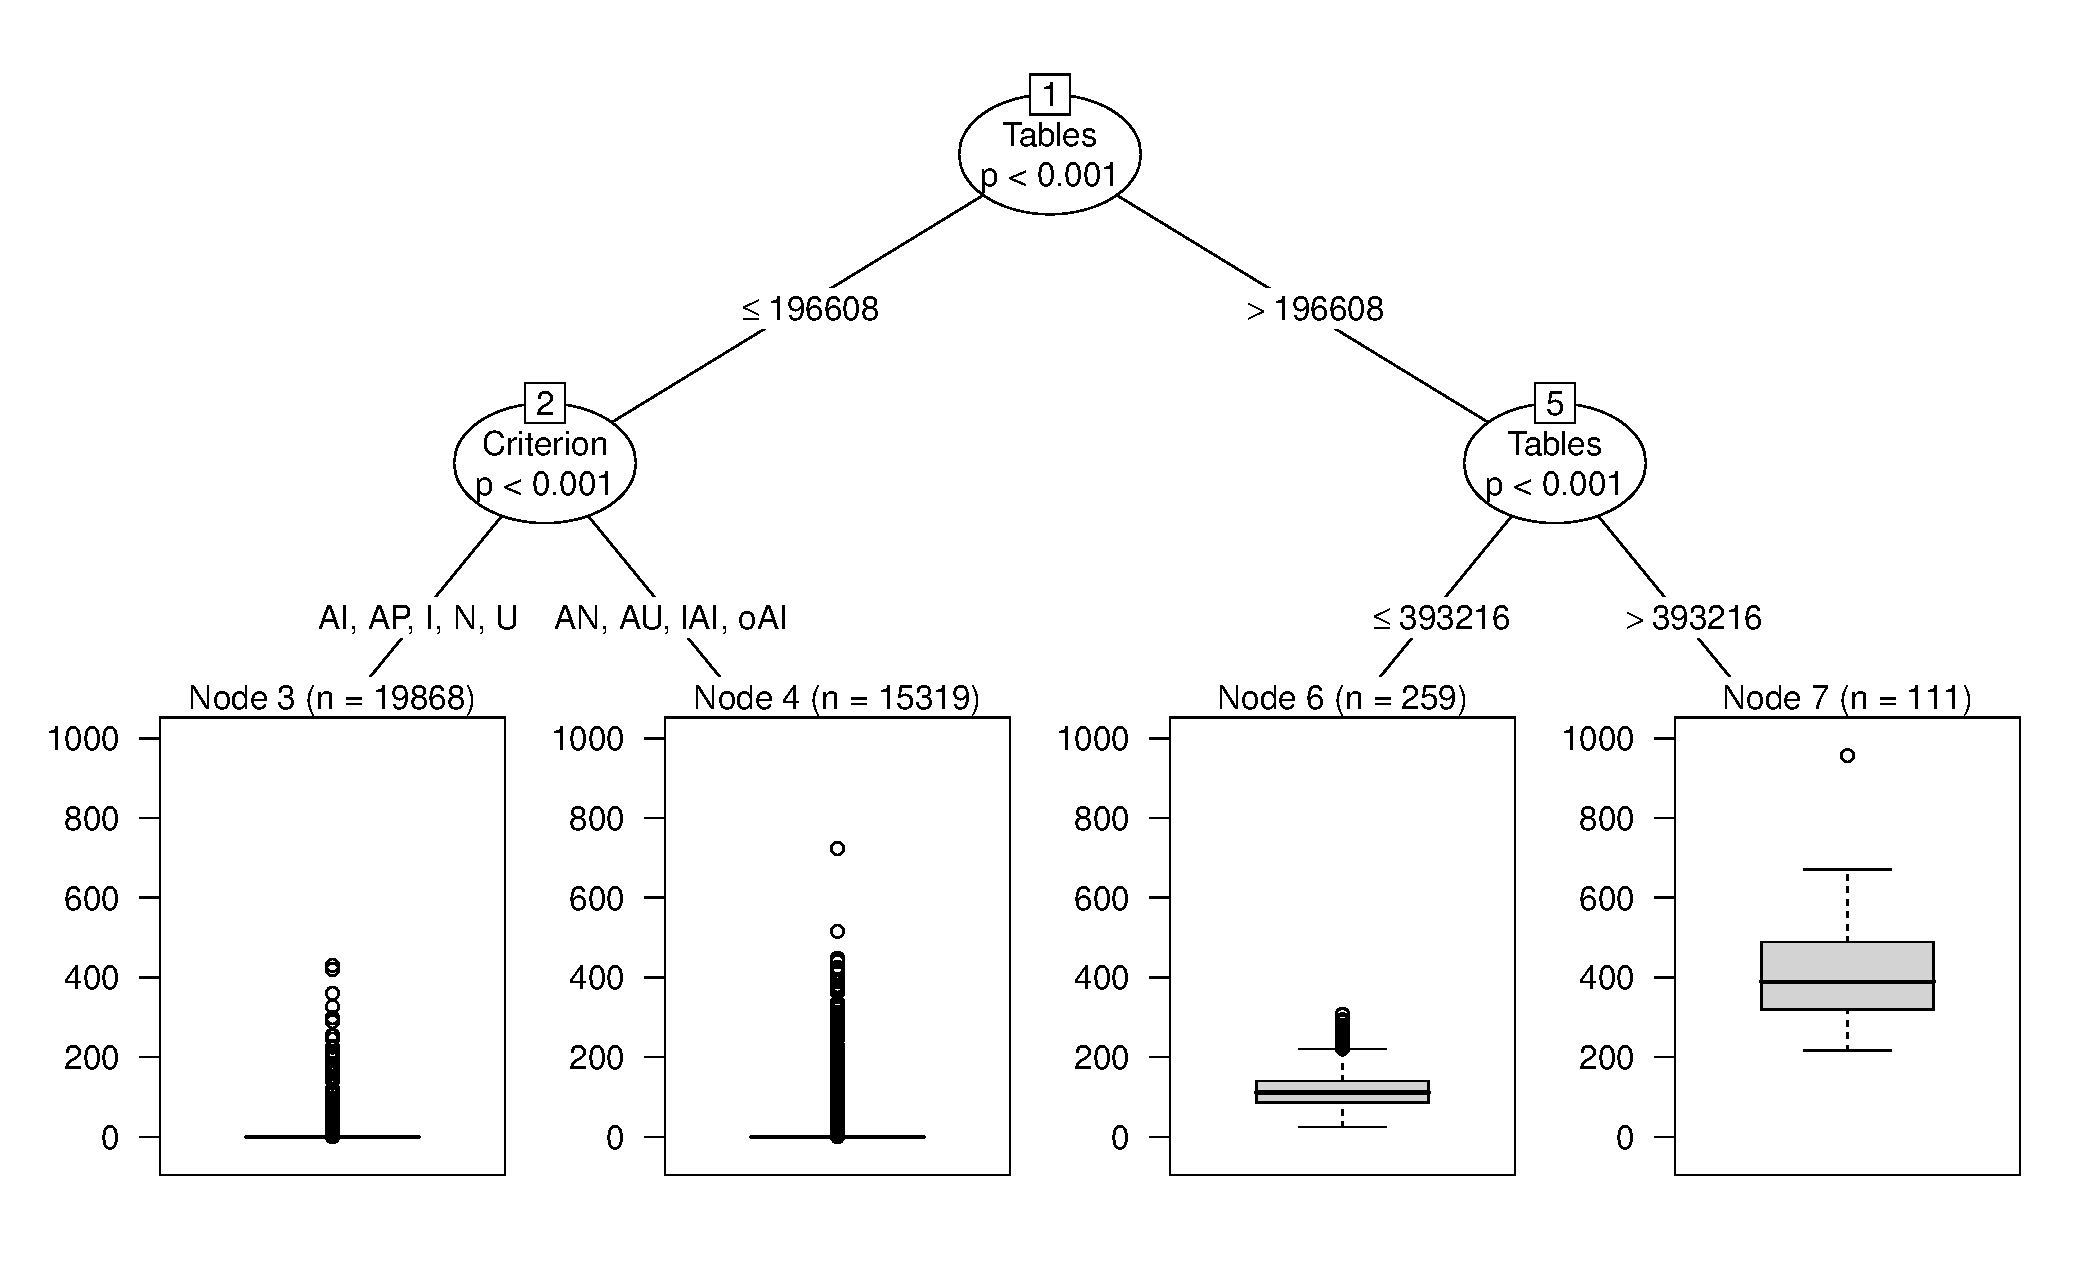
\includegraphics[width=.75\linewidth]{diagrams/AllTree.pdf}
  \caption{Regression tree using all variables to predict runtime in
  minutes. \vspace{-.15in}}
  \label{fig:atree}
  \vspace{-.15in}
\end{figure*}

\begin{figure*}
\centering
  \centering
  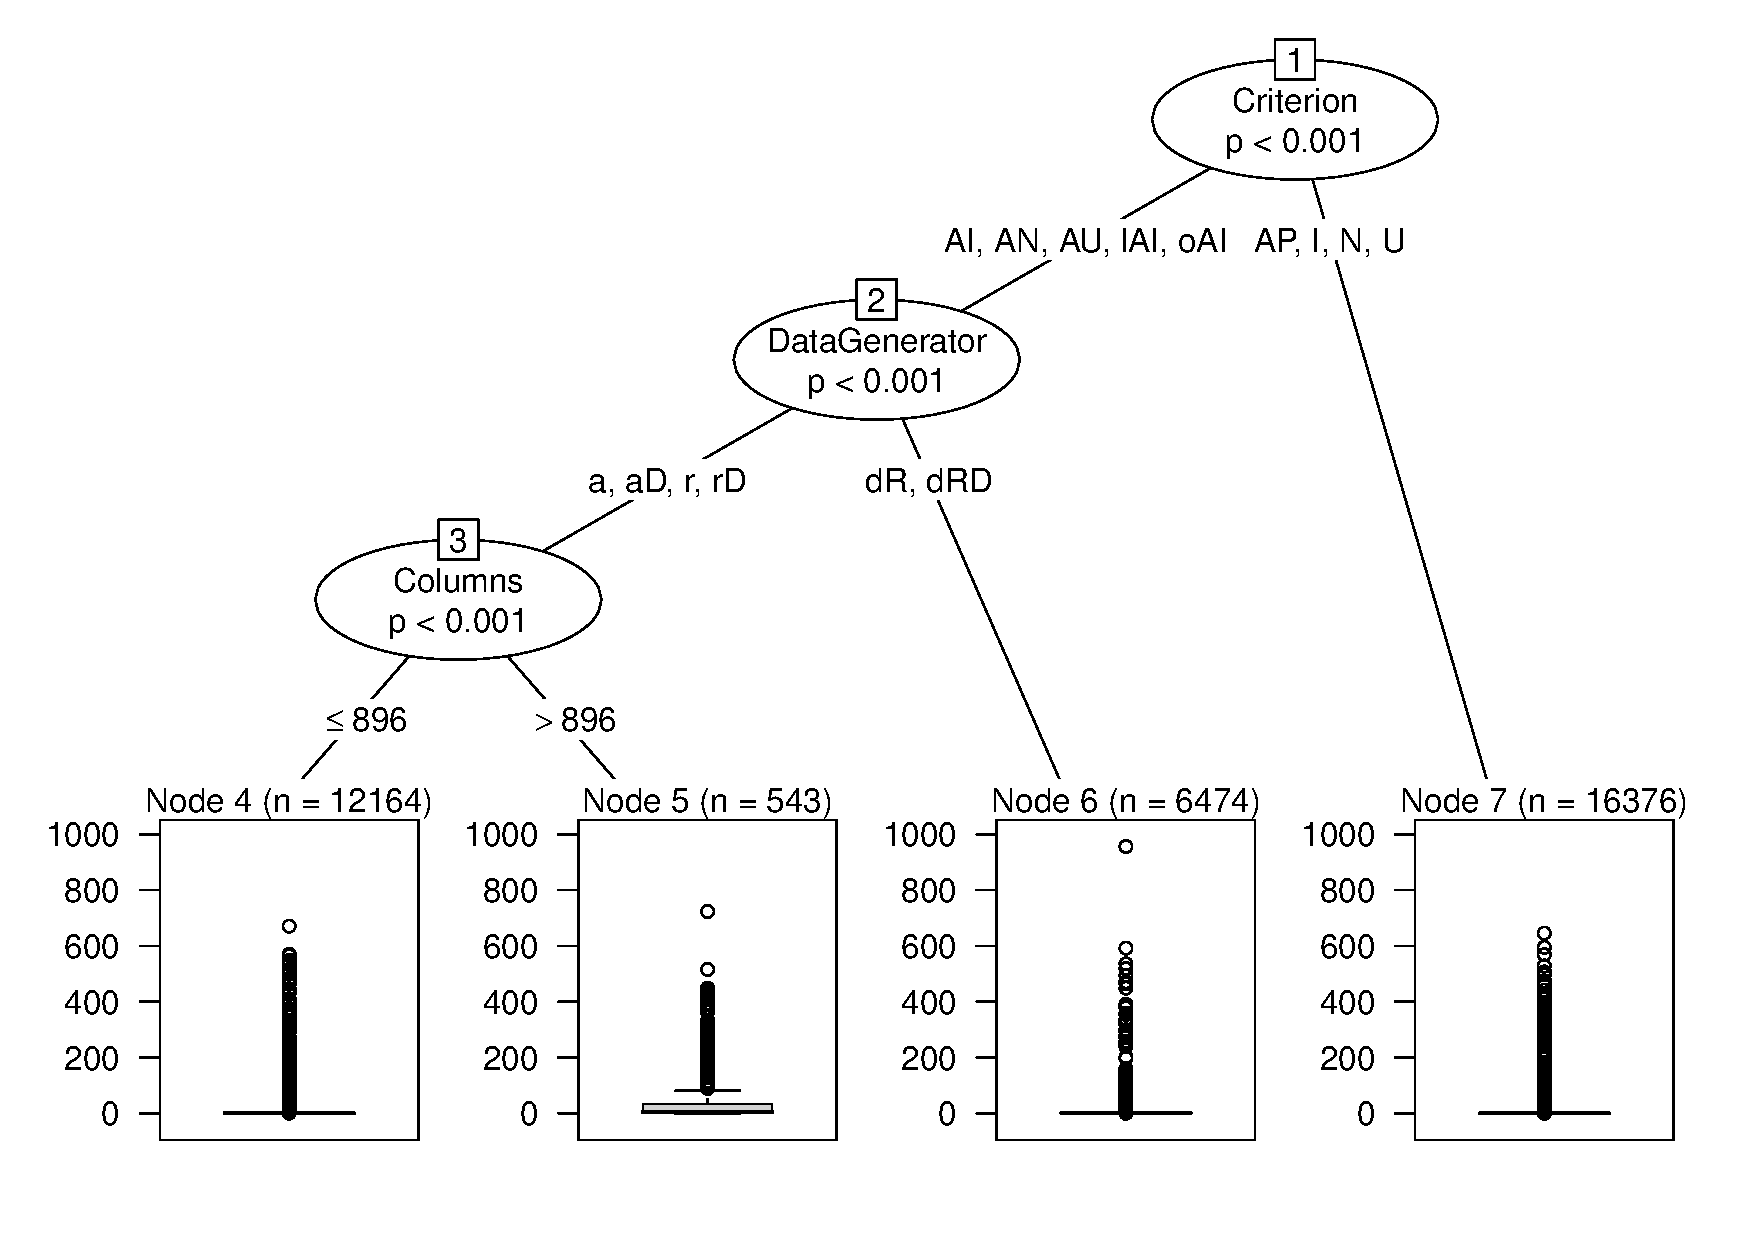
\includegraphics[width=.75\linewidth]{diagrams/NoTableCtreesd.pdf}
  \caption{Regression tree predicting runtime excluding Tables.\vspace{-.15in}}
  \label{fig:ttree}
  \vspace{-.15in}
\end{figure*}
